\newpage
\section{Korrektur}
\label{sec:Korrektur}

In Abbildung \ref{fig:einhuellende2} ist die Einhüllende nun bis zum rechten Rand
des Diagramms fortgesetzt. Eine Fortführung links der zeitlichen Nulllinie wird
als nicht sinnvoll erachtet, da der Entladevorgang des Kondensators erst ab $t=0$
beginnt.

\begin{figure}
  \centering
  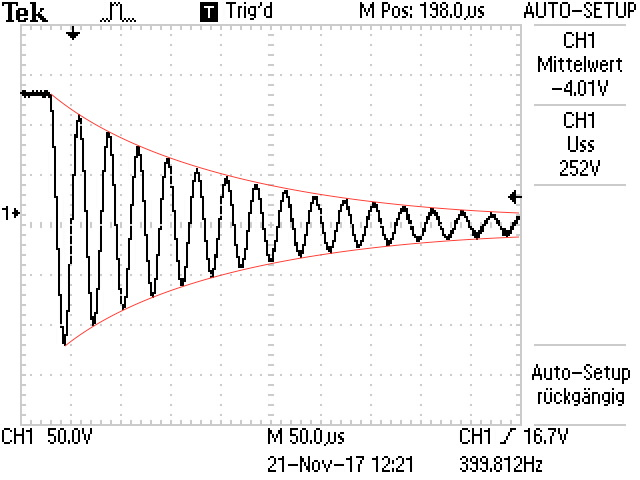
\includegraphics[width=300pt]{data/gedaempfte_schwingung2.JPG}
  \caption{Aufnahme des Spannungsverlaufs am Kondensator und Einhüllende bei der
  gedämpften Schwingung}
  \label{fig:einhuellende2}
\end{figure}

Die Theoriekurve für die Kondensatorspannung $U_{\symup{C}}$ in Abhängigkeit
von der Frequenz $f$ wird mit \eqref{eqn:Ucfrequenz} berechnet. Es ergibt sich die
in Abbildung \ref{fig:amplitudelog2} und \ref{fig:amplitudelin2} dargestellte
Theoriekurve.

\begin{figure}
  \centering
  \includegraphics[width=\textwidth]{build/amplitudelog.pdf}
  \caption{Halblogarithmische Auftragung der normierten Kondensatorspannung
  gegen die Frequenz}
  \label{fig:amplitudelog2}
\end{figure}

\begin{figure}
  \centering
  \includegraphics[width=\textwidth]{build/amplitudelin.pdf}
  \caption{Lineare Auftragung der normierten Kondensatorspannung gegen die
  Frequenz um den Resonanzbereich}
  \label{fig:amplitudelin2}
\end{figure}

Hier ist erkennbar, dass die Messwerte dem Verlauf der Theoriekurve in guter
Näherung folgen. Allerdings erreichen die Messwerte nicht die gleiche Höhe wie
die Theoriekurve und sind zudem relativ zu dieser leicht nach links verschoben.
Dies könnte auf Effekte der Schaltung, wie zum Beispiel nicht zu vernachlässigende
Widerstände von Kondensator und Spule, zurückzuführen sein.


Für die Berechnung der Theoriekurve für die Phasenverschiebung in Abhängigkeit
von der Frequenz wird die Formel
\begin{equation}
  \phi(\omega)=\arctan\biggl(\frac{L C \omega^2-1}{\omega R C}+\frac{\pi}{2}\biggr)\,.
\end{equation}
verwendet\footnote{Die in der Versuchsanleitung angegebene Formel \eqref{eqn:phase}
führt zu keinem sinnvollen Ergebnis. Zähler und Nenner wurden
vertauscht. Zudem muss noch die Phasenverschiebung am Kondensator berücksichtigt
werden.}.
Es ergibt sich die in Abbildung \ref{fig:philog2} und \ref{fig:philin2}
dargestellte Theoriekurve.


\begin{figure}
  \centering
  \includegraphics[width=\textwidth]{build/philog.pdf}
  \caption{Halblogarithmische Auftragung der Phasenverschiebung gegen die Frequenz}
  \label{fig:philog2}
\end{figure}

\begin{figure}
  \centering
  \includegraphics[width=\textwidth]{build/philin.pdf}
  \caption{Lineare Auftragung der Phasenverschiebung gegen die Frequenz}
  \label{fig:philin2}
\end{figure}

Es ist erkennbar, dass die Messwerte dem Verlauf der Theoriekurve für hinreichend
hohe Frequenzen $f$ in guter Näherung erfüllen. Die blau markierten Messwerte
sind als fehlerhaft zu bewerten.
